\section{Method}
\label{sec:method}

% Outline

% - select sample of urban areas (FUA)
%   - include only FUAs larger that 1 000 000 inhabitants to get a reasonable sample size
%   - get random 25 FUAs for each continent (or less if there is not enough large FUAs)
% - fetch the data from OSM
%   - download street networks
% - polygonize the network
% - measure shape charactersitics
%     - measure initally more than Reock (get a sample from ESDA)
%     - there is a conceptual backbone to this - we know that the artifacts are either
%       small (small intersections) polygons or can be large but then they are very
%       narrow (in between dual carriegaway)
%     - we need a shape metric that captures this relationship
% - identify optimal measurements
%     - plots that help us visually detect a cluster of artifacts
% - derivation of 1-dimensional index
%     - from Roeck and area we can derive one value from which distribution we can
%       identify a cut-off value for artifact/non-artifact polygons
% - cut-off value detection
% - exploration of geographical variation
%     - differences between cities and continents
% - open tools, open data, open code with full reproducibility

Make a strong case for the fact that our method is very simple (it is not a machine
learning algorithm); computationally cheap; AND manages to capture BOTH elongated
bananas and intersection bananas with ONE stroke and ONE index, which is possible thanks
to the CHARACTERISTIC PATTERNS in urban street networks. As demonstrated in the scatter
plot \ref{fig:banana-scatter}...

\begin{figure}
    \centering
    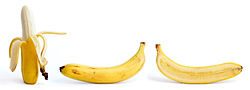
\includegraphics{figures/banana}
    \caption{[Show shape index v. area plot for different continents (?) or for
    different FUA(s) to show the banana shape in the distribution]}
    \label{fig:banana-scatter}
\end{figure}

\subsection*{Method section on using shape indeces}
mention Sanzana \cite{sanzana_decomposition_2018}, Louf \cite{louf_typology_2014}, ...
etc.


\textit{Sanzana et al. propose an algorithm for identification and elimination of
``bad-shaped polygons'', incl. streets/roads/footpaths. Explain that while we have
a comparable approach, we are concerned with *cities* while they are concerned
with *hydrological models*; and since cities express some certain regularities
we can make use of that}

\subsection*{Method section on finding the minimum and using it as a threshold
(put part of this in results maybe?)}

\begin{figure}
    \centering
    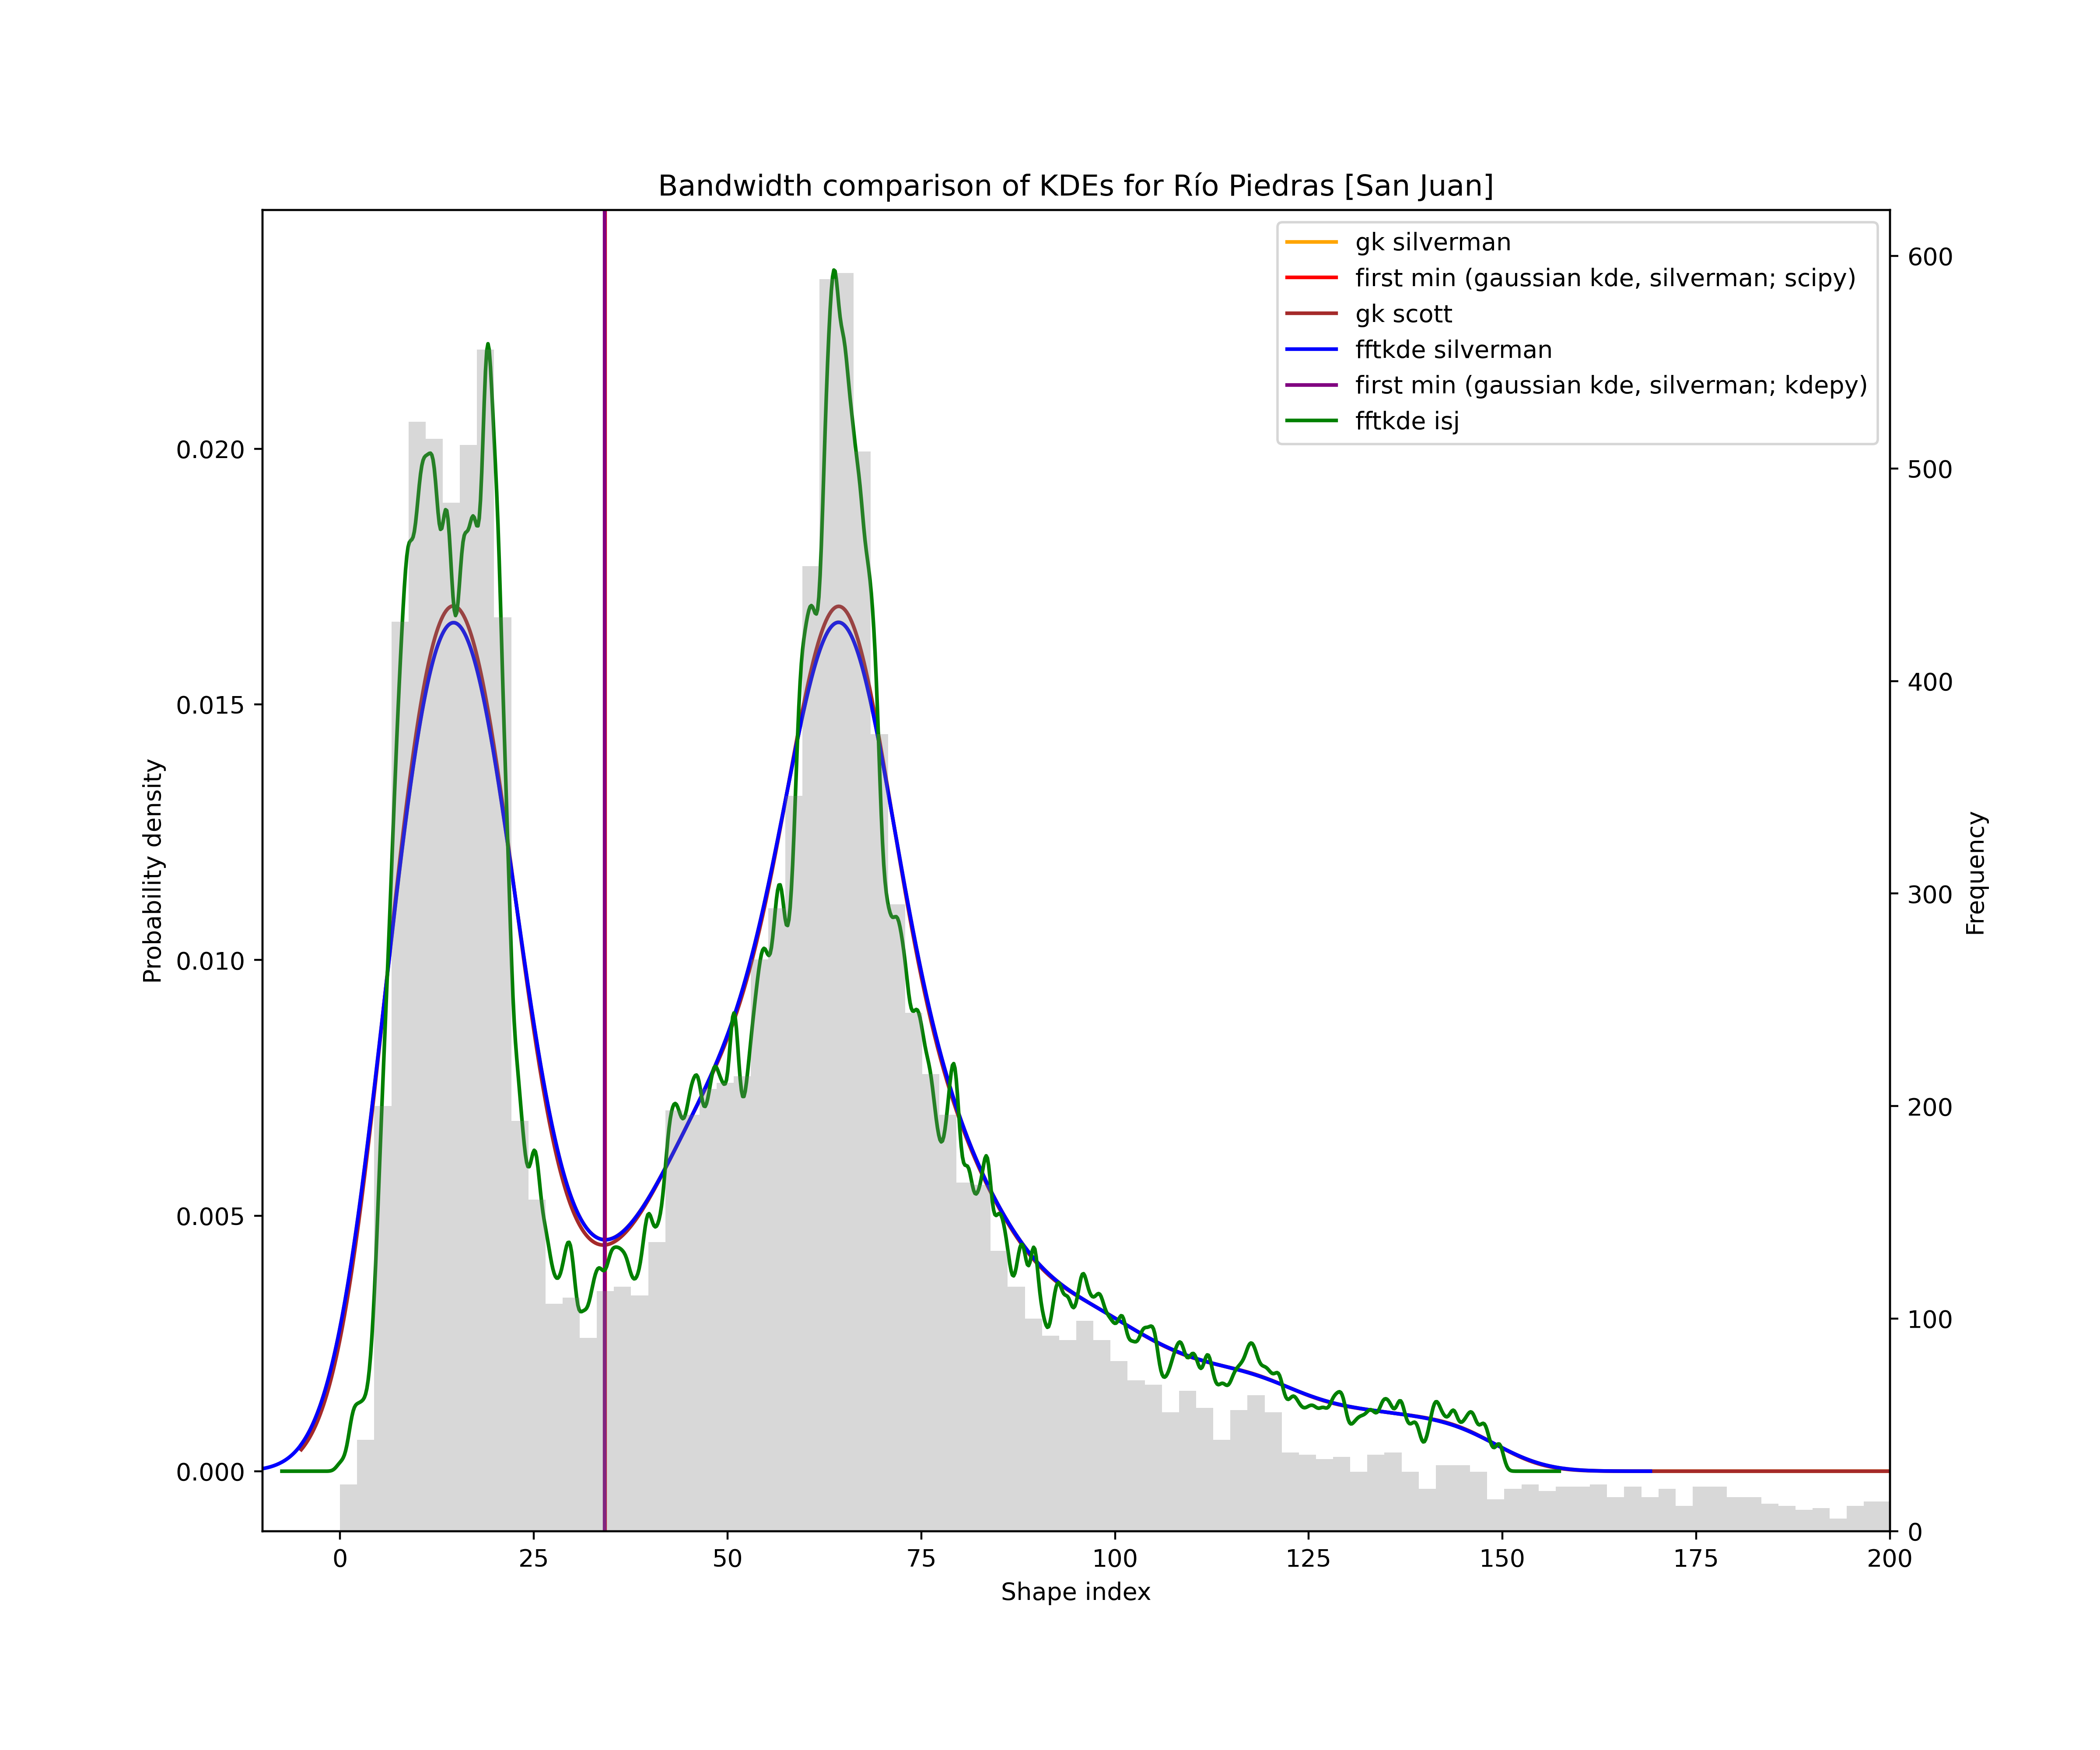
\includegraphics[width=0.5\linewidth]{figures/308}
    \caption{[Above: just a placeholder. Insert here: shape index frequency d
    istribution(s) for FUA X. - show the two-peak pattern]}
    \label{fig:si-dist}
\end{figure}

Many, though not all, shape index frequency distributions for the analyzed FUAs reveal a
common feature of two prominent peaks (see Figure \ref{fig:si-dist}). Through visual
analysis, we find that these peaks represent two different types of polygons. Most of
the polygons from the first (leftmost) peak can be attributed to ``bananas’’ in the
street network, whereas most of the polygons from the second (rightmost) peak represent
true urban blocks. Therefore, for FUAs that show a pronounced two-peak pattern in their
shape index frequency distribution, the minimum \textit{between} the two peaks can be
used as shape index threshold: polygons with a shape index below the threshold will most
likely be ``bananas’’; polygons with a shape index above the threshold will most likely
be true urban blocks. To derive the minimum, we approximate the shape index frequency
distribution with a Gaussian kernel density estimation. For bandwidth selection, we use
the parametric Silverman method \cite{silverman_using_1981} and find that it gives
satisfactory results; non-parametric bandwidth selection methods might be a subject for
future work (see section \ref{sec:discussion}).

Next, comparing the positions of peak 1, peak 2, and shape index threshold for different
FUAs with pronounced two-peak patterns, we find that maxima positions vary to a
considerably greater extent than minima positions. In other words, shape index
thresholds for ``banana’’ identification from morphologically different FUAs lie within
a relatively narrow range. We therefore hypothesize that applying a shape index
threshold within the range identified from FUAs whose polygons follow a two-peak
distribution will allow the identification of ``bananas’’ polygons even for those FUAs
whose distributions do not show a two-peak pattern. Applying the … [TBD: lower
boundary/median/average/higher boundary] of the empirically derived shape index
threshold range to the rest of FUAs indeed reveals ``bananas´´ polygons in all/most FUAs
(see Figure \ref{fig:city}).